


\section{Time graph of different meteorological variables}
\label{sec-1}


There is a variety of scientific researches interested in the
relationship between several meteorological variables. A suitable
approach is to display the time evolution of all of them either
using a panel for each of the variables or plotting them
superposed. The superposition of variables with different ranges
is not very useful (unless their values were previously rescaled),
so this option is postponed for later use. 

For this example we will use the daily data from the SIAR
meteorological station located at Aranjuez (Madrid). The code of
the province (28) and station (3) is extracted from
\url{http://solar.r-forge.r-project.org/data/SIAR.csv}. Let's download a
multivariate time series of eight years of daily data from January
2004 to December 2011. 



    


  

  
  
  



  

This multivariate time series can be directly displayed with the
\texttt{xyplot} method of \texttt{lattice} using the \texttt{layout} argument to
display the variables with parallel panels arranged in rows.


\lstset{language=R}
\begin{lstlisting}
xyplot(aranjuez, layout=c(1, ncol(aranjuez)))
\end{lstlisting}

\begin{figure}[htb]
\centering
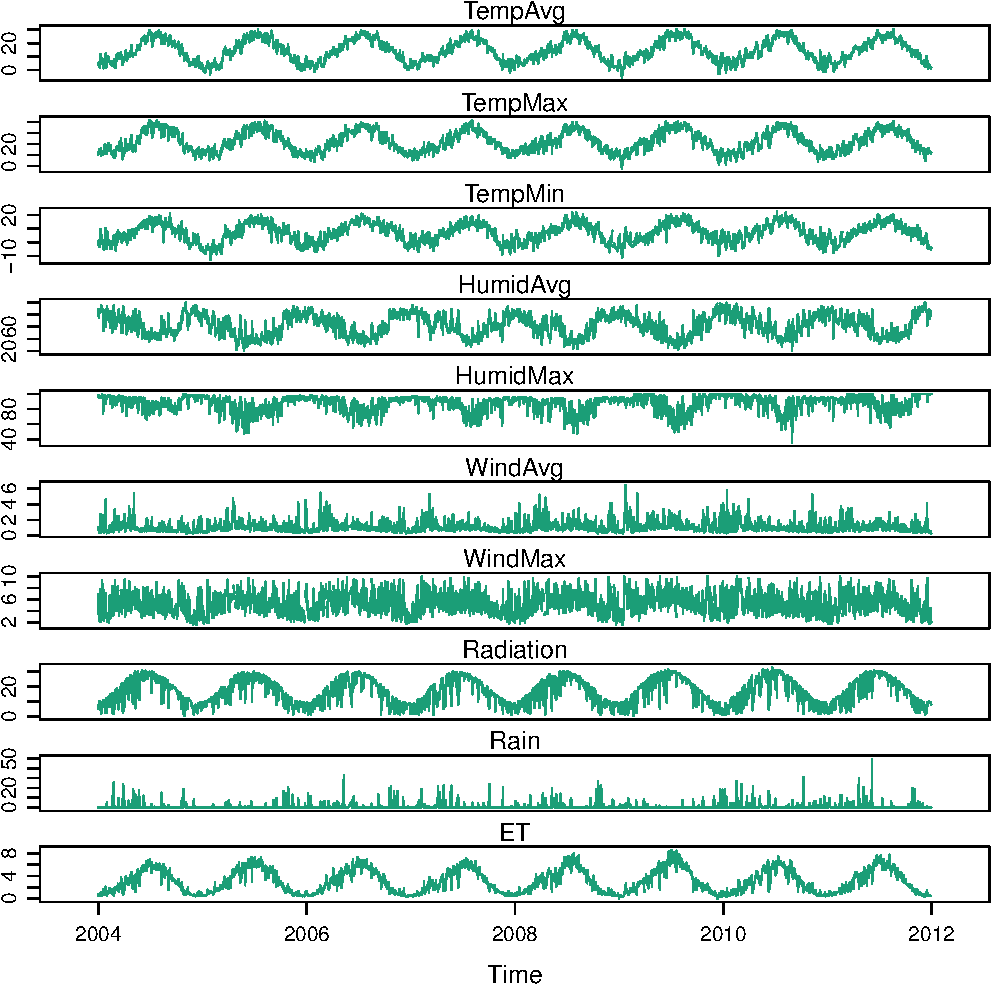
\includegraphics[width=.9\linewidth]{figs/aranjuez.pdf}
\caption{\label{fig:aranjuezNaive}Time plot of the collection of meteorological time series of the Aranjuez station.}
\end{figure}

This first attempt can be improved with a custom panel
function. This function will generate the content of each panel
using the information processed by \texttt{xyplot}. Since these functions
are executed consecutively, the order of the functions determines
the superposition of information:
\begin{itemize}
\item The label of each time series is displayed with text inside each
  panel instead of using the strips mechanism. The \texttt{panel.text}
  prints the name of each variable with the aid of \texttt{panel.number}.
\item The alternation of years is displayed with blocks of gray and
  white color using the \texttt{panel.xblocks} function from
  \texttt{latticeExtra}. The year is extracted (as character) from the
  time index of the \texttt{zoo} object with \texttt{format.POSIXlt}.
\item Those values below the mean of each variable are highlighted
  with short red color blocks at the bottom of each panel, again
  with the \texttt{panel.xblocks} function.
\item The maxima and minima are hihglighted with blue small triangles.
\end{itemize}

\index{Panel function}
\index{panel.xblocks@\texttt{panel.xblocks}}
\index{panel.text@\texttt{panel.text}}
\index{panel.number\texttt{panel.number}}
\index{panel.points\texttt{panel.points}}

\lstset{language=R}
\begin{lstlisting}
Year <- function(x)format(x, "%Y")

xyplot(aranjuez, layout=c(1, ncol(aranjuez)), strip=FALSE,
       scales=list(y=list(cex=0.6, rot=0)),
       panel=function(x, y, ...){
         panel.xblocks(x, Year, col = c("lightgray", "white"),
                       border = "darkgray")
         panel.xblocks(x, y<mean(y, na.rm=TRUE), col = "indianred1",
                       height=unit(0.1, 'npc'))
         panel.xyplot(x, y, ...)
         panel.text(x[1], min(y, na.rm=TRUE),
                    names(aranjuez)[panel.number()],
                    cex=0.7, pos=2,...)
         idxMax <- which.max(y)
         panel.points(x[idxMax], y[idxMax], col='black', fill='lightblue', pch=24)
         idxMin <- which.min(y)
         panel.points(x[idxMin], y[idxMin], col='black', fill='lightblue', pch=25)
       })
\end{lstlisting}

\begin{figure}[htb]
\centering
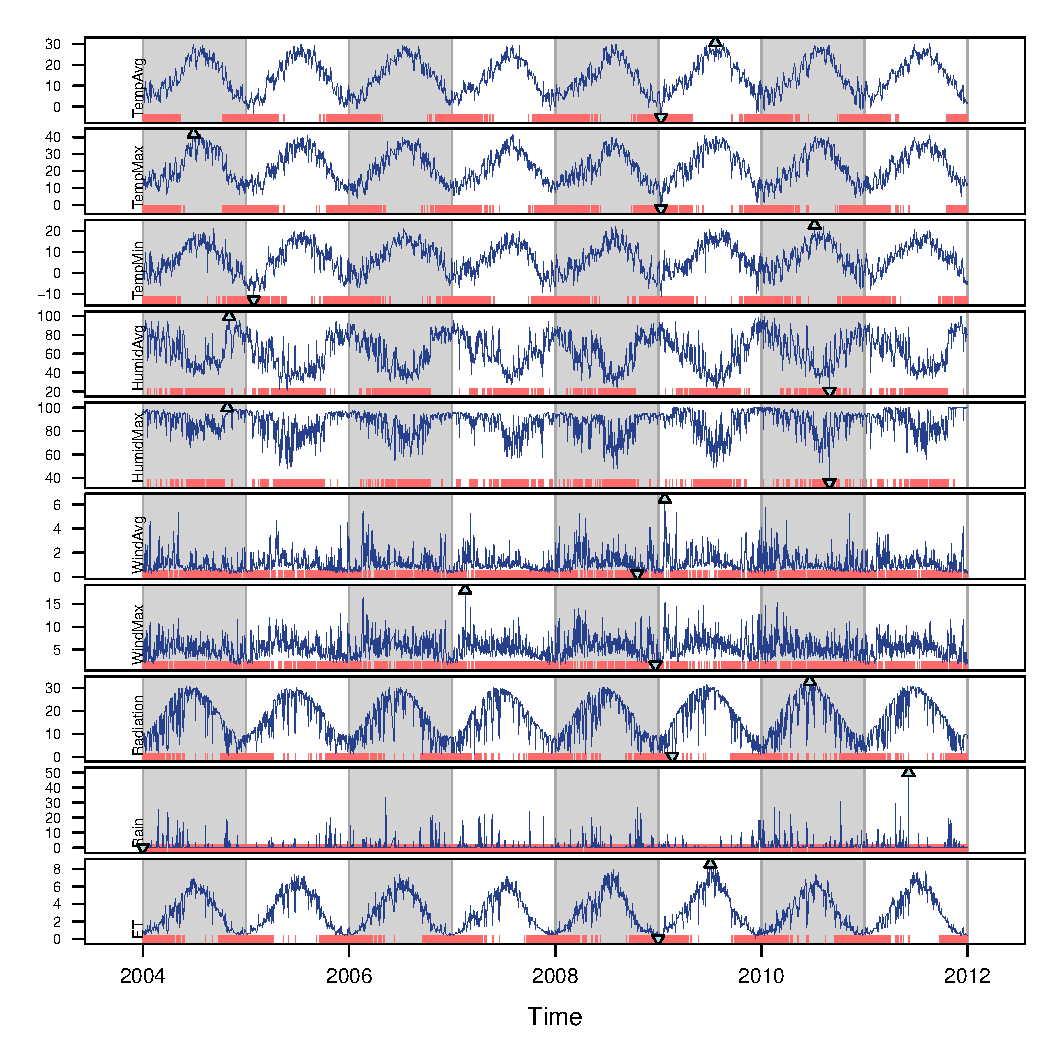
\includegraphics[width=.9\linewidth]{figs/aranjuezXblocks.pdf}
\caption{\label{fig:aranjuezEnhanced}Enhanced time plot of the collection of meteorological time series of the Aranjuez station.}
\end{figure}
\section{Confronting variables: the scatter plot matrix}
\label{sec-2}


But, what if instead of displaying the time evolution we want to
confront the variables between them? Then a matrix of scatter
plots is the answer. This graphical tool is implemented in the
\texttt{splom} function. 

\index{splom@\texttt{splom}}

\lstset{language=R}
\begin{lstlisting}
colors <- c(brewer.pal(n=11, 'RdBu'), '#000000')
colors <- colors[c(6:1, 12:7)]

splom(~as.data.frame(aranjuez),
      groups=format(index(aranjuez), '%m'),
      auto.key=list(space='right', 
        title='Month', cex.title=1),
      pscale=0,
      par.settings=custom.theme(symbol=colors,
        pch=19), cex=0.3, alpha=0.1)
\end{lstlisting}

\begin{figure}[htb]
\centering
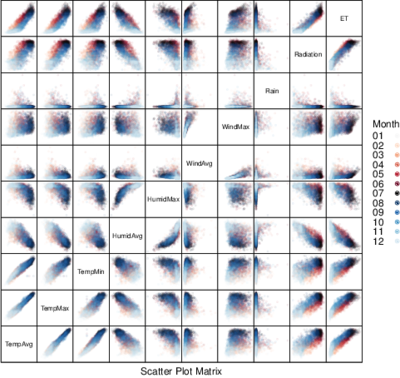
\includegraphics[width=.9\linewidth]{figs/aranjuezSplom.pdf}
\caption{\label{fig:aranjuezSplomNaive}Scatter plot matrix of the collection of meteorological time series of the Aranjuez station.}
\end{figure}

However, for large datasets, the display of a large number of
points in a scatter plot matrix produces hidden point density,
long computation times and slow displays. These problems can be
circumvented with the estimation and representation of points
densities.  A common encoding uses gray scales, pseudo colors or
partial transparency. An improved scheme encodes density as the
size of hexagon symbols inscribed within hexagonal binning region
\cite{Carr.Littlefield.ea1987}.

The \texttt{hexbin} package includes several functions for hexagonal
binning.  The \texttt{panel.hexbinplot} is a good substitute for the
default panel function. Besides, our first attempt with \texttt{splom}
can be improved with several modifications:
\begin{itemize}
\item The scales ticks and labels are suppressed with \texttt{pscale=0}.
\item The panels of the lower part of the matrix (\texttt{lower.panel}) will include a
  locally weighted scatterplot smoothing (loess) with
  \texttt{panel.loess}.
\item The diagonal panels (\texttt{diag.panel}) will display the kernel
  density estimate of each variable. The \texttt{density} function
  computes this estimate. The result is adjusted to the panel
  limits (calculated with \texttt{current.panel.limits}). The kernel
  density is plotted with \texttt{panel.lines} and the \texttt{diag.panel.splom}
  function completes the content of each diagonal panel (since
  \texttt{pscale=0} this function only generates the label of each variable).
\item The point density is encoded with the palette \texttt{BTC} (ligther
  colors for high density values and darker colors for almost
  empty regions, with a gradient of blue hues for intermediate values).
\end{itemize}

\index{Packages!hexbin@\texttt{hexbin}}
\index{panel.hexbinplot@\texttt{panel.hexbinplot}}
\index{panel.loess@\texttt{panel.loess}}
\index{diag.panel.splom@\texttt{diag.panel.splom}}
\index{current.panel.limits@\texttt{current.panel.limits}}
\index{Panel function}

\lstset{language=R}
\begin{lstlisting}
library(hexbin)

splom(~as.data.frame(aranjuez),
           panel=panel.hexbinplot, xlab='',
           colramp=BTC,##function(n)BTC(n, beg=250, end=5),
           diag.panel = function(x, ...){
             yrng <- current.panel.limits()$ylim
             d <- density(x, na.rm=TRUE)
             d$y <- with(d, yrng[1] + 0.95 * diff(yrng) * y / max(y))
             panel.lines(d)
             diag.panel.splom(x, ...)
           },
           lower.panel = function(x, y, ...){
             panel.hexbinplot(x, y, ...)
             panel.loess(x, y, ..., col = 'red')
           },
           pscale=0, varname.cex=0.7
           )
\end{lstlisting}

\begin{figure}[htb]
\centering
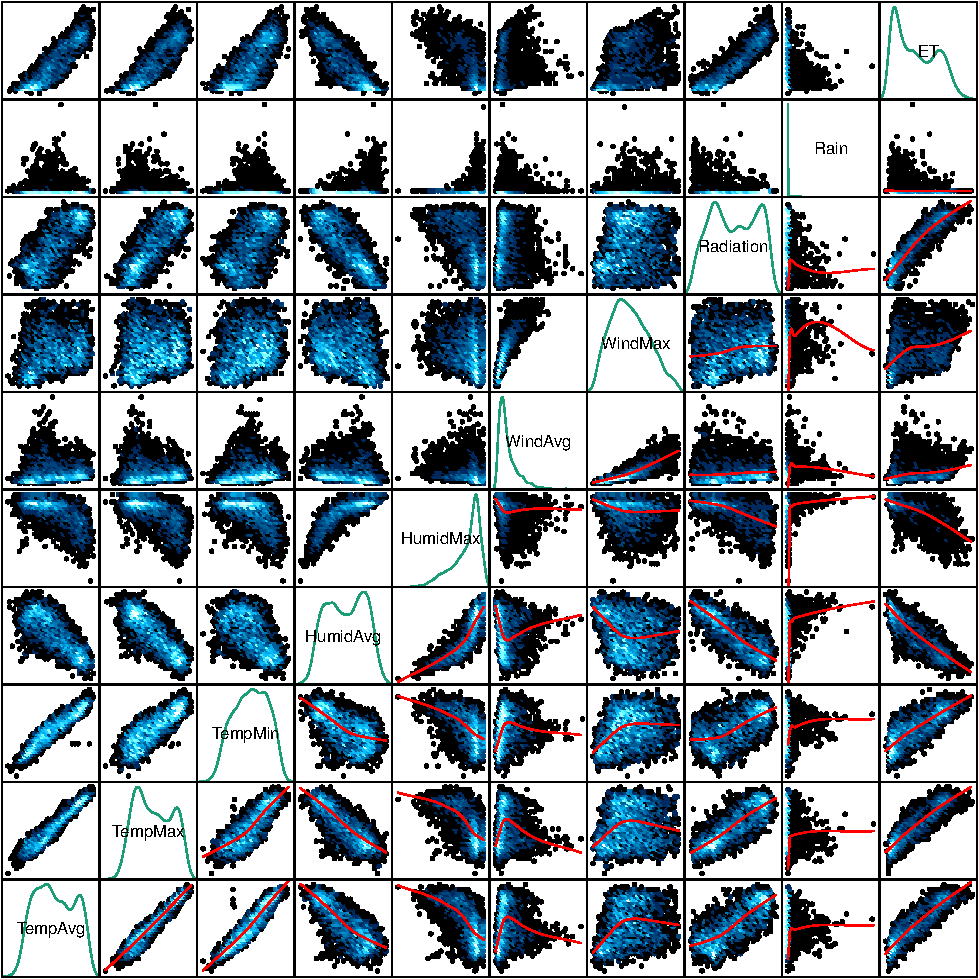
\includegraphics[width=.9\linewidth]{figs/aranjuezSplomHexbin.pdf}
\caption{\label{fig:aranjuezSplomHexbin}Scatter plot matrix of the collection of meteorological time series of the Aranjuez station using hexagonal binning.}
\end{figure}

Let's add a bit of interactivity to this plot with the
identification of some points. This task is easy with
\texttt{panel.link.splom}. The points are selected via mouse clicks (and
highlighted in green). Clicks other than left-clicks terminate the
procedure. The output of this function is the index of chosen points.

\index{panel.link.splom@\texttt{panel.link.splom}}
\index{trellis.focus@\texttt{trellis.focus}}

\lstset{language=R}
\begin{lstlisting}
trellis.focus('panel', 1, 1)
idx <- panel.link.splom(pch=13, cex=0.6, col='green')
aranjuez[idx,]
\end{lstlisting}


A drawback of the matrix of scatter plots is that each panel is drawn
independently so it is impossible to compute a common color key
for all of them. In other words, two cells with exactly the same
color in different panels encode different points densities. 

It is possible to display a reduced set of variables against
another one and generate a common color key using the \texttt{hexbinplot}
function. First, the dataset must be reshaped from the wide format
(one colum for each variable) to the long format (only one column for
the values with one row for each observation). 

The \texttt{reshape} function needs several arguments to perform the
conversion. The most important is the \texttt{data.frame} to be
transformed. Then there is the names of variables to be mapped to
a single variable in the long dataset (the three ambient
temperatures). The name of this variable can be set with
\texttt{v.names}. Finally, \texttt{timevar} is the name of the column in long format that
differentiates multiple observations from the same variable. The
values of this column are defined with the \texttt{times} argument.

\index{reshape@\texttt{reshape}}

\lstset{language=R}
\begin{lstlisting}
aranjuezDF <- data.frame(aranjuez,
                         month=format(index(aranjuez), '%m'))
aranjuezRshp <- reshape(aranjuezDF, direction='long',
                        varying=list(names(aranjuez)[1:3]),
                        v.names='Temperature',
                        times=names(aranjuez)[1:3],
                        timevar='Statistic')
\end{lstlisting}


\lstset{language=R}
\begin{lstlisting}
head(aranjuezRshp)
\end{lstlisting}


\begin{verbatim}
Error en grid.Call.graphics(L_downviewport, name$name, strict) : 
  Viewport 'subpanel.7.-108' was not found
     TempAvg TempMax TempMin HumidAvg HumidMax WindAvg WindMax Rain Radiation
     ET
          HumidAvg HumidMax WindAvg WindMax Rain Radiation        ET month
1.TempAvg     88.3     95.9   0.746   3.528    0     5.490 0.5352688    01
2.TempAvg     83.3     98.5   1.078   6.880    0     6.537 0.7710499    01
3.TempAvg     75.0     94.4   0.979   6.576    0     8.810 0.8361229    01
4.TempAvg     82.0     97.0   0.633   3.704    0     9.790 0.6861381    01
5.TempAvg     83.2     97.0   0.389   2.244    0    10.300 0.5152422    01
6.TempAvg     84.5     96.5   0.436   2.136    0     9.940 0.4886631    01
          Statistic Temperature id
1.TempAvg   TempAvg       4.044  1
2.TempAvg   TempAvg       5.777  2
3.TempAvg   TempAvg       5.850  3
4.TempAvg   TempAvg       4.408  4
5.TempAvg   TempAvg       3.081  5
6.TempAvg   TempAvg       2.304  6
\end{verbatim}

The \texttt{hexbinplot} displays this dataset with a different panel for
each type of temperature (average, maximum and minimum) but with a
common color key encoding the point density. Now, two cells with
the same color in different panels encode the same value.

\index{hexbinplot@\texttt{hexbinplot}}
\index{Panel function}

\lstset{language=R}
\begin{lstlisting}
hexbinplot(Radiation~Temperature|Statistic, data=aranjuezRshp,
           layout=c(1, 3), colramp=BTC, 
           panel=function(x, y, xlim,...){
             panel.hexbinplot(x, y, ...)
             panel.loess(x, y, ..., col = 'red')
           }
           )
\end{lstlisting}

\begin{figure}[htb]
\centering
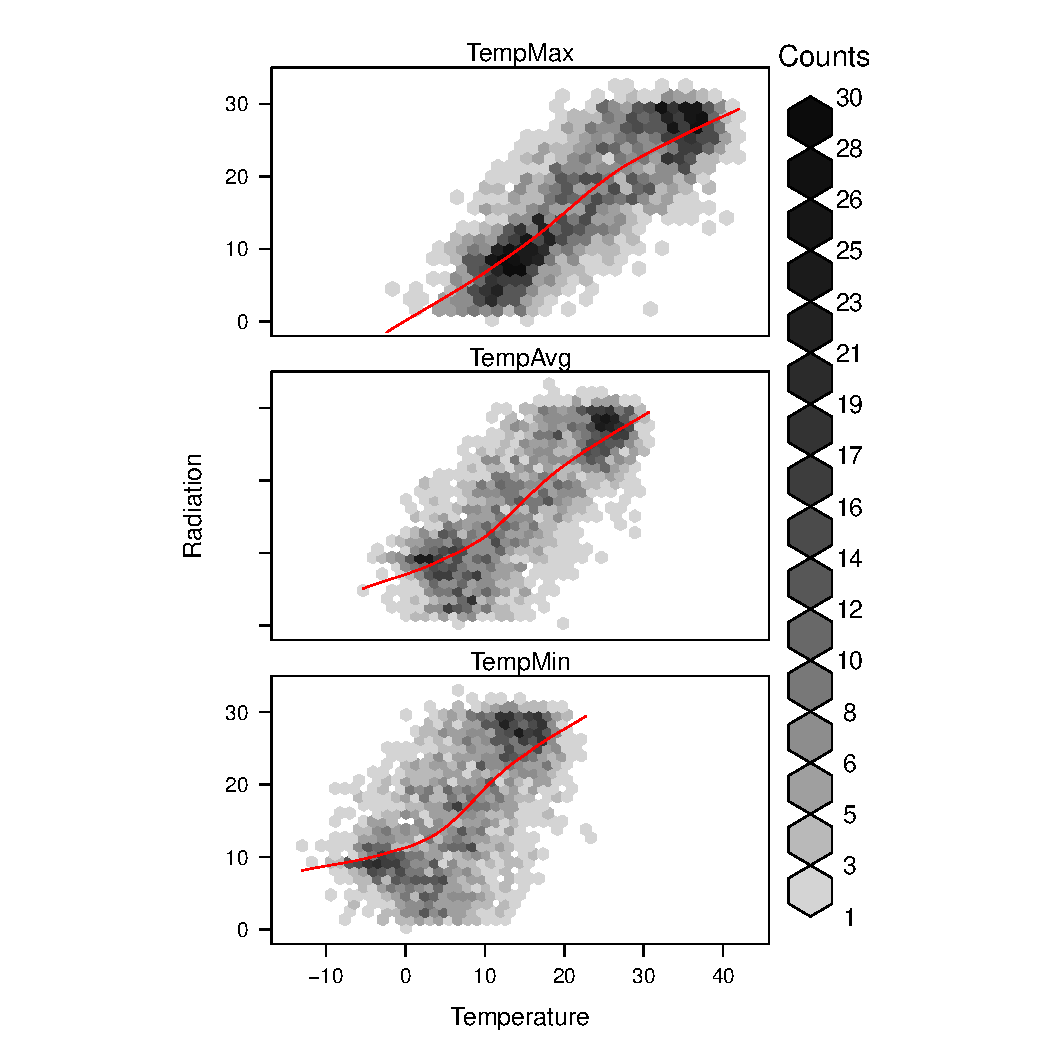
\includegraphics[width=.9\linewidth]{figs/aranjuezHexbinplot.pdf}
\caption{\label{fig:aranjuezHexbin}Scatter plot with hexagonal binning of temperature versus solar radiation using data of the Aranjuez station.}
\end{figure}


\index{useOuterStrips@\texttt{useOuterStrips}}
\index{panel.rug@\texttt{panel.rug}}
\index{panel.loess\texttt{panel.loess}}
\index{Packages!latticeExtra@\texttt{latticeExtra}}

\lstset{language=R}
\begin{lstlisting}
useOuterStrips(xyplot(Temperature~Radiation|month*Statistic,
                      data=aranjuezRshp,
                      between=list(x=0), 
                      panel=function(...){
                        panel.xyplot(...,
                                     col='skyblue4', pch=19,
                                     cex=0.5, alpha=0.3)
                        panel.rug(..., col.line='indianred1',
                                  end=0.05, alpha=0.6)
                        panel.loess(..., col='indianred1', lwd=1.5)
                        }))
\end{lstlisting}

\begin{figure}[htb]
\centering
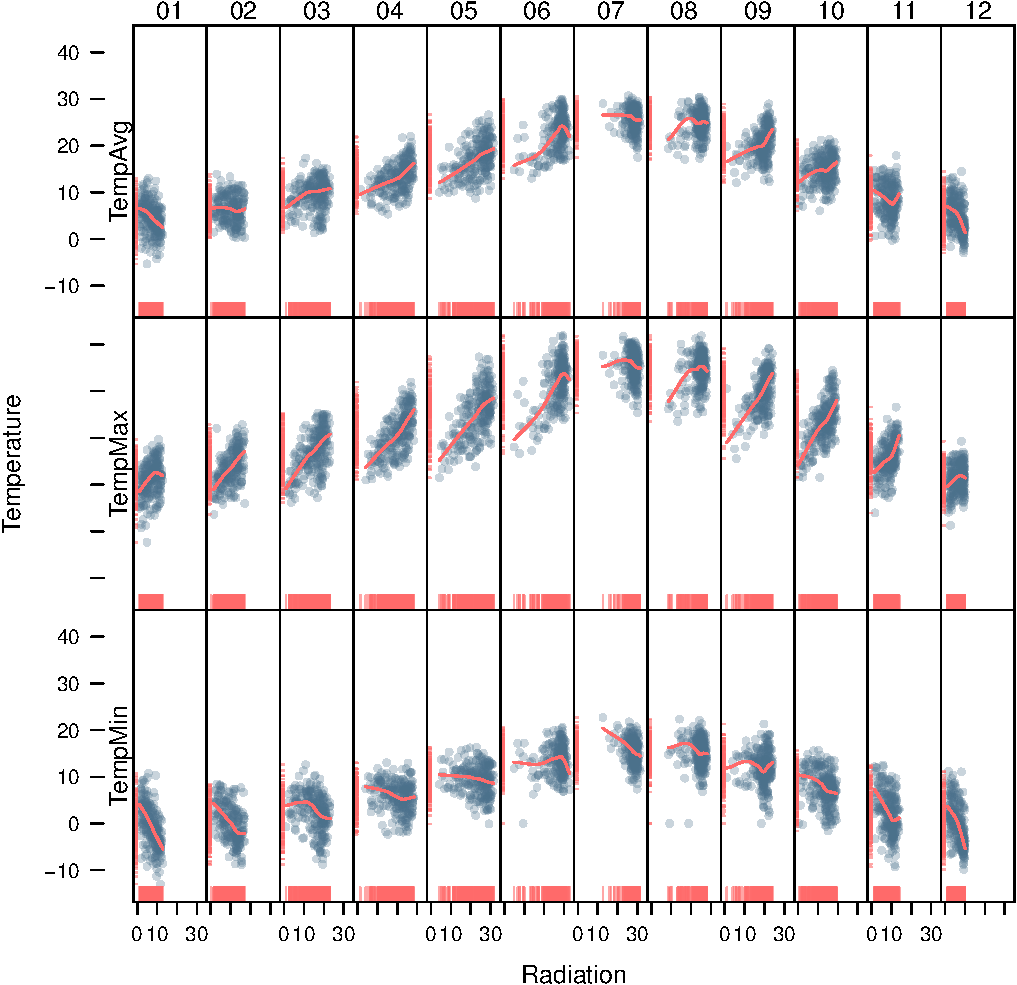
\includegraphics[width=.9\linewidth]{figs/aranjuezOuterStrips.pdf}
\caption{\label{fig:aranjuezOuterStrips}Scatter plot of temperature versus solar radiation for each month using data of the Aranjuez station.}
\end{figure}
